\chapter{相关基础理论框架}

\section{卷积神经网络与网络训练}
卷积神经网络(CNN:Convolutional Neural Neural Network)最早由LeCun于1989年提出\cite{Zhou.etal2017},Krizhevsky等人于2012年成功将深度卷积神经网络运用在了图像处理方面的实验,并且性能指标远远超过了支持向量机等传统机器学习方法,并对计算机视觉领域产生了十分深远的影响。本小节简要介绍神经网络中的卷积运算和池化方式。

\subsection{卷积运算与池化}
卷积操作是卷积神经网络(CNN)的核心组成部分,它通过参数共享的卷积核对输入数据进行局部线性加权。池化操作是一种利用特定位置邻域的综合统计信息来替代该位置输出的方法。例如,在最大池化(Max Pooling)中,会选取邻域内的最大值作为该位置的输出;而在均值池化(Average Pooling)中,则会取邻域内的平均值作为该位置的输出。除此之外,还有诸如L²范数池化、依距离中心远近进行加权平均的池化等多样化的池化函数可供选择。当对空间区域实施池化操作时,网络能够获得对输入少量平移的一定不变性,即即便对输入数据进行细微平移,经池化操作后的网络输出基本能保持稳定。此外,池化操作还具备对特征降维的优势,这样一来,既能够减轻网络的计算负担,又在一定程度上有助于防止过拟合现象的发生,进而便于网络的优化过程。具有以下显著特点:

\subsubsection{局部连接}
与传统神经网络的全连接方式不同,卷积操作在空间上采用局部连接,输出与输入之间的连接是局部且稀疏的。这种局部连接可以通过较小的卷积核尺寸来实现。在深度卷积神经网络中,多层卷积操作的堆叠使得网络深层的单个神经元能够与大部分输入(感受野范围内的输入)间接连接,从而高效地捕捉输入与输出之间的复杂关系。



\subsubsection{参数共享}
在卷积神经网络中,卷积核的参数在输入的不同空间位置上是共享的。这意味着只需要学习一组卷积核参数,而不需要为每个位置单独学习一组参数。这种参数共享机制大幅减少了模型参数量,降低了存储需求,同时提升了模型的计算效率。


\subsubsection{平移等边}
先对输入数据进行平移变换,再实施卷积操作,与先进行卷积运算后再对结果进行平移,两者所得的输出结果具有一致性。这一特性表明,卷积操作能够有效捕捉和定位输入数据中特定特征的位置。然而,对于图像的缩放、旋转等几何变换,卷积操作并不具备类似的等变性,需要借助其他特定的机制或网络结构来处理这些变换。


\subsubsection{感兴趣池化区域}

过去,图片里有多个感兴趣区域时,先裁剪再输入卷积神经网络提取特征效率低下。RoI Pooling的出现,改变了这一现状,它允许同一图片的多个感兴趣区域共享底层特征。具体操作是,先将整张图片输入卷积神经网络,得到整张图的特征图。之后,把感兴趣区域映射到特征图对应位置。再依据设定的输出维度,把映射后的区域划分为相同大小的子区域,子区域数量与输出维度一致。最后,对每个子区域进行最大池化操作。经此流程,所有感兴趣区域特征维度相同,与输入图片大小、感兴趣区域大小无关。



\subsubsection{位置敏感的感兴趣区域池化}

池化操作赋予网络一定的平移不变性,通常网络深度越大,这种不变性越显著,这对于物体分类任务具有积极作用。然而,在目标检测任务中,对图片中的物体进行精确定位时,需要网络能够感知位置信息,此时平移不变性反而会带来不利影响。为了解决这个问题,Dai等人提出了一种位置敏感的感兴趣区域池化方法,该方法在特征提取过程中引入了相对位置信息。通过使用不同的卷积核通道来提取不同位置上的特征信息,有效地提升了卷积神经网络在处理物体位置信息方面的能力。这种改进使得网络在保持对物体分类的有效性的同时,也能够更好地应对目标检测任务中对物体位置精确感知的需求。


\subsection{网络训练}
深度学习本质上是一种基于数据驱动的机器学习方法,其核心在于借助训练数据来调整网络内部的参数,这一点对于深度学习算法的成功至关重要。在本小节中着重介绍了两种网络训练的基础算法:反向传播与随机梯度下降。具体内容如下:

\subsubsection{反向传播}

深度学习中的反向传播(BP:Back Propagation)算法基于微积分中的链式法则,用于计算复合函数的导数。该算法将网络输出层的损失函数中得到的梯度信息,沿着网络连接路径反向传播回网络的各个前层,从而得到各层网络参数对损失函数的梯度,用于优化网络参数。通过链式法则,可以直接得出网络中任一参数相对于损失函数的梯度的代数表达式。然而,在计算这种表达式时,需要考虑是采用一次性计算并存储的方式,还是进行多次重复计算。为了减少重复计算,可能需要增加存储空间。在内存不足的情况下,可以通过多次重复计算来节省内存。




\subsubsection{随机梯度下降}


使用梯度下降法优化网络参数是一种有效的方法。具体来说,梯度下降法通过将参数沿着损失函数在该参数处的导数的反方向移动一小步,从而减小损失函数的值。随机梯度下降(SGD: Stochastic Gradient Descent)是其中最常用的算法之一。其核心思想是利用小批量样本的平均梯度来近似估计整个训练集的梯度期望值。每次网络更新的计算仅在训练集中采样的小批量样本上进行。对于固定的批量大小,随机梯度下降算法收敛所需的更新次数通常与训练集的样本数成正相关。



\section{多目标跟踪数据集}

\subsection{MOT数据集}

MOT数据集是多目标跟踪领域的重要基准数据集,本文主要在MOT数据集上进行测试,分别是MOT-16\cite{Mahmoudi.etal2019}、MOT-17\cite{Sun.etal2021}和MOT-20数据集\cite{Yan.etal2022}。如图\ref{fig:np101}所示,是MOT数据集部分视频序列的采样帧示例。

\begin{figure}[htbp] % 可以是h(here),t(top),b(bottom),p(page of floats)
	\centering
	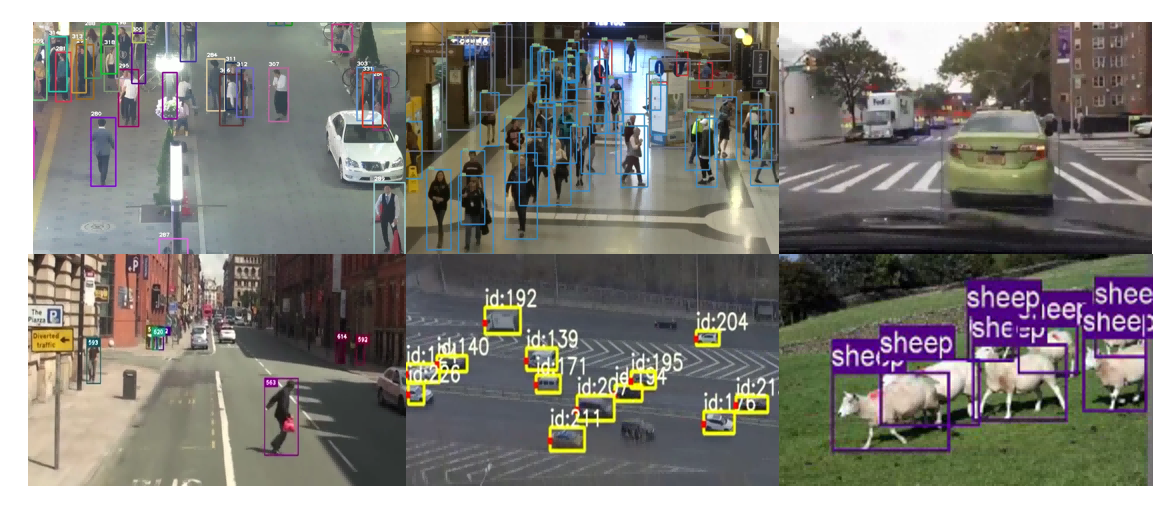
\includegraphics[width=1\textwidth]{np101} % 假设图片文件名为car.pdf或car.png等,位于当前工作目录
	\caption{MOT数据集部分视频序列的采样帧示例} % 图片标题
	\label{fig:np101} % 用于引用的标签
\end{figure}


\subsubsection{MOT-16数据集}
MOT-16数据集于2016年发布,是MOT Challenge系列的一部分,用于衡量多目标检测跟踪方法标准的数据集,主要关注行人跟踪。主要包含训练集和测试集。训练集有7个子目录,每个子目录对应一段视频的抽帧图片及标注,且带有 ground truth,能为训练模型提供关键参考;测试集数据结构类似,但没有 ground truth,主要用于算法性能的独立评估。数据中的每一帧都以单独图片文件形式存储,便于按序处理和分析 。标注信息存储在文本文件中,每行代表一次检测事件,各字段以逗号分隔,涵盖物体类别、边界框坐标等重要参数,可用于模型训练和结果验证。

自从MOT-16数据集2016年开发以来主要用于多目标跟踪算法的研究、开发和评估。研究人员用其训练和优化算法模型,对比不同算法在该数据集上的表现,分析算法的优势与不足,进而改进算法。在智能视频监控领域,通过在 MOT-16 数据集上训练的算法,可实现对行人的精准跟踪,为公共安全保障、人群流量分析等提供技术支持 。在自动驾驶场景中,有助于开发更可靠的行人检测和跟踪系统,提高自动驾驶安全性。





\subsubsection{MOT-17数据集}
MOT-17 数据集是 MOT Challenge 系列的一部分,由苏黎世联邦理工学院、阿德莱德大学及达姆施塔特工业大学联合创办 ,旨在评估不同算法在复杂场景下的多目标跟踪性能,主要聚焦于行人跟踪任务。该数据集于2017年发布,继承并扩展了MOT15和MOT16的特点,在原有框架基础上增加了新挑战,推动了多目标跟踪技术的研究进展。

MOT-17数据集包含多个视频序列,这些序列均来自真实世界的监控摄像头拍摄的视频片段,涵盖了多种城市环境。每个视频序列都有对应的图像文件,所有帧按时间顺序编号并保存为 JPEG 格式。每个视频序列都有相应的标注文件,以 CSV 格式存储。





\subsubsection{MOT-20数据集}

MOT-20数据集于2020年由德国慕尼黑工业大学的Dynamic Vision and Learning Group发布,关注人群密集的场景。主要包含8个视频片段,分别来自火车站、城镇广场、体育场等不同场景,4个用于训练,4个用于测试。总共包含13410帧,训练视频8931帧,测试视频4479帧。

主要运用在智能安防监控中助力人流密集场所安全管理与异常行为监测,在智能交通系统用于行人过街辅助和交通流量分析,在商业领域服务店铺运营与商场客流分析,还为学术研究提供算法研发与技术融合的评估支撑。




作为MOT数据集,MOT-16、MOT-17和MOT-20三者评估指标基本是一致的,以下便是具体内容:

MOTA综合考虑了漏检、误报以及身份切换错误等多种因素,是衡量多目标跟踪算法性能的重要指标。计算方法为\[MOTA = 1 - \frac{\sum_{t} fp_{t}+m_{t}+mme_{t}}{\sum_{t} g_{t}}\]其中\(\sum_{t} fp_{t}\)是虚警数,\(\sum_{t} m{t}\)是漏警数,\(\sum_{t} g{t}\)t是所有帧中真实标注轨迹的数量,\(\sum_{t} mme{t}\)是身份交换数,MOTA 得分越接近 1,表示算法性能越好。

MOTP(:用于测量平均位置精度,反映检测边界框与实际标注之间的重叠程度。通过计算所有成功匹配的目标与其对应真值之间距离误差的均值来衡量,公式为\[
MOTP = \frac{\sum_{i,j} d(i,j) \cdot I(d(i,j) < thr)}{\left| \{(i,j) | I(d(i,j) < thr) = 1\} \right|}
\]其中d(i,j)表示第i帧内预测轨迹j和其最接近的真实实例间的欧氏距离,thr是设定的判断有效关联的阈值。

IDF1 Score:结合了识别率(IDR)和召回率(FDR),通过 F-measure 将两者结合形成最终评分,公式为\[
IDF1 = 2\times\frac{IDR\times FDR}{IDR + FDR}
\]该指标用于评估算法在目标身份识别和跟踪过程中的准确性。


\subsection{PETS-2009}


\subsubsection{PETS-2009介绍}
PETS-2009\cite{ferryman2009pets2009}数据集曾是视频多目标跟踪领域广泛运用的数据集之一。该数据集涵盖了三个针对不同任务的子集:

S1:用于人群计数与密度估计;

S2:用于行人跟踪;

S3:用于人流分析和事件识别。

在这些子集中,与视频多目标跟踪关联较为紧密的是 S2 子集。其包含三个视频序列如图\ref{fig:np102}所示:

\begin{figure}[htbp] % 可以是h(here),t(top),b(bottom),p(page of floats)
	\centering
	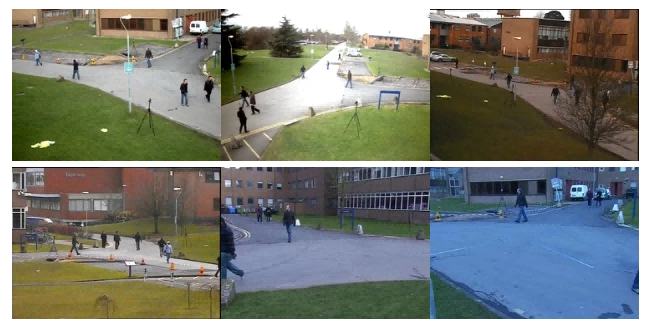
\includegraphics[width=1\textwidth]{np102} % 假设图片文件名为car.pdf或car.png等,位于当前工作目录
	\caption{PETS-2009数据集中S2子集三个视频序列的采样帧示例} % 图片标题
	\label{fig:np102} % 用于引用的标签
\end{figure}

S2L1:属于相对简单的视频序列,平均每帧约有五名行人。当下多数先进的多目标跟踪算法在 S2L1 上均可达成超 90\% 的精度。因此,对于这一视频序列,若继续深挖性能提升,意义或许有限,因为这有致使过拟合的风险;

S2L2:这是一个具有中等密度的视频序列,平均每帧约有二十名行人;

S2L3:这是一个高密度的视频序列,平均每帧约有四十名行人。

PETS-2009 数据集在过去是视频多目标跟踪领域中广受欢迎的资源。然而,其使用过程中存在一些不规范的问题。首先,PETS 2009 研讨会所公布的数据集使用说明并不要求使用者在所有视频序列上对其算法进行测试。这导致许多已发表的方法仅在部分序列上进行评估,从未在完整数据集上进行全面测试,使得我们难以判断这些方法展示的结果是否具有足够的代表性。

其次,该数据集的组织者并未发布真实标注,而是通过每年举办研讨会,邀请研究人员提交算法的跟踪结果供组织者评估。在研讨会之外,其他算法所报告的跟踪结果往往难以进行公平的比较。除了选择性地使用视频序列外,研究人员可能还采用了独立的真实标注,并使用了不同的检测输入和评价指标。

另外,PETS-2009 数据集的所有视频序列均拍摄于相同的场景,且摄像机位置固定,背景变化幅度较小,仅有轻微的光照变化。数据集未涵盖由移动摄像机拍摄的场景,其背景变化幅度较大。

这些问题凸显了多目标跟踪领域对多样化数据集基准及标准化评估指标的迫切需求,后续内容将对此作进一步探讨。

\subsubsection{性能指标}
准确率,计算分类正确的样本数占总样本数的比例,是衡量分类模型整体正确性的基础指标。
\[Accuracy = \frac{TP+TN}{TP+TN+FP+FN}\]

召回率,反映正样本被正确识别的能力,适用于关注样本总体情况的场景。
\[\text{Recall} = \frac{TP}{TP + FN}\]

平均精度均值,所有类别平均精度的平均值,综合评价目标检测模型在多类别上的性能。
\[mAP = \frac{1}{n} \cdot \sum_{i=1}^{n} AP_i\]

成功跟踪率,衡量目标跟踪算法在跟踪过程中成功跟踪目标的比例,是目标跟踪任务中的重要指标。
\[Success\ Rate = \frac{\text{成功跟踪的帧数}}{\text{总帧数}}\]